\documentclass{article}
\usepackage{booktabs}
\usepackage{amsmath}
\usepackage{amssymb}
\usepackage[noend]{algorithmic}
\usepackage[nothing]{algorithm}
\usepackage{tikz}
\usepackage{latexsym}
\usepackage{float}
\providecommand{\e}[1]{\ensuremath{\times 10^{#1}}}
\renewcommand{\thealgorithm}{}
\title{CS 521: Data Structures and Algorithms I \\ Extra Credit 2}
\author{Dustin Ingram}
\begin{document}
\maketitle
\begin{enumerate}
    \item \textbf{(23-1) Solution:} 
    \begin{enumerate}
        \item Since every edge in the undirected, connected graph $G(V,E)$ is unique, this means that when creating the MST, there must be a unique light edge across every cut of the graph, regardless of how the cut is made, which results in a unique MST. The second-best spanning tree, however, will not necessarily be unique, as can be shown by the following example:\\
        \begin{figure}[H]
        \centering
        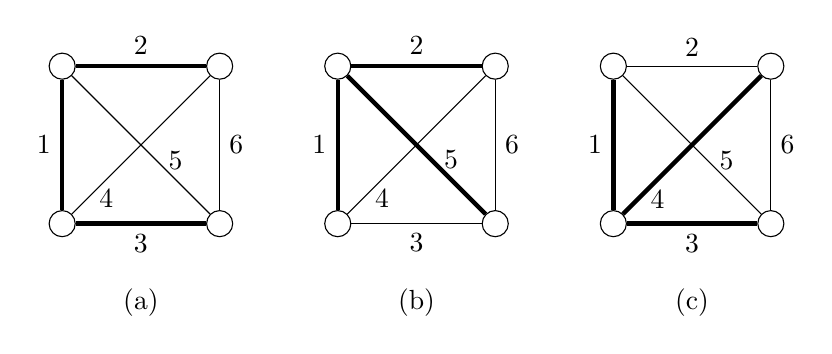
\begin{tikzpicture}[]
        \begin{scope}
          \node[draw,shape=circle]     (a) at (0,0) {};
          \node[draw,shape=circle]     (b) at (2,0) {};
          \node[draw,shape=circle]     (c) at (0,-2) {};
          \node[draw,shape=circle]     (d) at (2,-2) {};
          \node at (1,-3) {(a)};

          \draw[ultra thick] (a) -- (b) node[midway, above] {2};
          \draw[ultra thick] (a) -- (c) node[midway, left] {1};
          \draw (b) -- (d) node[midway, right] {6};
          \draw[ultra thick] (c) -- (d) node[midway, below] {3};
          \draw (a) -- (d) node[near end, above] {5};
          \draw (b) -- (c) node[near end, below] {4};
        \end{scope}

        \begin{scope}[xshift=3.5cm]
          \node[draw,shape=circle]     (a) at (0,0) {};
          \node[draw,shape=circle]     (b) at (2,0) {};
          \node[draw,shape=circle]     (c) at (0,-2) {};
          \node[draw,shape=circle]     (d) at (2,-2) {};
          \node at (1,-3) {(b)};

          \draw[ultra thick] (a) -- (b) node[midway, above] {2};
          \draw[ultra thick] (a) -- (c) node[midway, left] {1};
          \draw (b) -- (d) node[midway, right] {6};
          \draw (c) -- (d) node[midway, below] {3};
          \draw[ultra thick] (a) -- (d) node[near end, above] {5};
          \draw (b) -- (c) node[near end, below] {4};
        \end{scope}

        \begin{scope}[xshift=7cm]
          \node[draw,shape=circle]     (a) at (0,0) {};
          \node[draw,shape=circle]     (b) at (2,0) {};
          \node[draw,shape=circle]     (c) at (0,-2) {};
          \node[draw,shape=circle]     (d) at (2,-2) {};
          \node at (1,-3) {(c)};

          \draw (a) -- (b) node[midway, above] {2};
          \draw[ultra thick] (a) -- (c) node[midway, left] {1};
          \draw (b) -- (d) node[midway, right] {6};
          \draw[ultra thick] (c) -- (d) node[midway, below] {3};
          \draw (a) -- (d) node[near end, above] {5};
          \draw[ultra thick] (b) -- (c) node[near end, below] {4};
        \end{scope}

        \end{tikzpicture}
        \end{figure}
        Here, (a) is the minimum spanning tree of total weight $W=6$, while (b) and (c) are the second-best MSTs, each with weight $W=8$. We see that with this configuration, the second-best MST is not unique.

        \item If $T$ is the MST of $G$ such that $(u,v) \in T$ and $(x,y) \notin T$, let the second-best MST of $G$ be $T_{2}$ such that $T_{2} = \{T - (u,v)\} \cup \{(x,y)\}$. If we consider the graph of $T \cup T_{2}$, there will be one cycle in the graph, and the edges $(u,v)$ and $(x,y)$ will be on the cycle. By definition, $w(u,v) < w(x,y)$ must be true, otherwise we could replace $(u,v)$ with $(x,y)$ in $T$ to produce an MST with a lower weight. Therefore we see that $T$ is the lowest-weight MST, and that $T$ and $T_{2}$ differ by only one edge.
        \item For every pair of vertices $(u,v)$ in the graph, the path $u \leadsto v$ is a unique simple path. This means that we can simply do a DFS (or, BFS) search from every vertex $u \in G.V$, storing the maximum traversed edge for each pair of vertices $(u,v)$. Since we are determining the maximum for all pairs $(u,v)$ in the graph, we discover $V^{2}$ total edges for a runtime of $O(V^2)$.
        \item As previously established, finding the second-best MST $T^{2}$ requires replacing one edge $(x,y)$ in the MST $T$ with one edge $(u,v) \notin T$. This means that for every path $\{u \leadsto v\} \cup (u,v)$, we produce a cycle, and must remove the maximum edge that is not $(u,v)$. Since we can produce an MST in at least $O(V^{2})$ time, and use the algorithm described in (c) to compute the maximum-edge for every path in $O(V^{2})$ time, the remaining problem becomes finding a path $u \leadsto v$ in $T$ and an edge $(u,v) \notin T$ such that
        $$w(u,v) - w(\textsc{Max}(u \leadsto v))$$
        is minimized; once $(u,v)$ is found, the second best MST is
        $$T^{2} = \{T - \textsc{Max}(u \leadsto v)\} \cup (u,v)$$
        The minimization simply requires examining every edge $\notin T$, therefore the overall runtime is guaranteed to be $O(V^2)$.
    \end{enumerate}
    
    \item \textbf{(15-1) Solution:} 
    Given a DAG $G(V,E)$ with edge weights $w \in \mathbb{R}$ and to vertices $s$ and $t \in G.V$, we must find the longest weighted simple path $s \leadsto t$. 
    \begin{algorithm}[H]
    \floatname{algorithm}{\normalfont\textsc{Longest-DAG-Path}$(G, w, s, t, u)$}
    \caption{}
    \begin{algorithmic}
        \IF{$u == s$}
            \STATE $s.\pi = \textsc{Nil}$
            \FOR{each vertex $v \in G.V$}
                \STATE $v.w = 0$
            \ENDFOR
        \ELSIF{$u == t$}
            \STATE $r = [u]$
            \WHILE{$u \neq \textsc{Nil}$}
                \STATE $r.\textsc{Push}(u.\pi)$
                \STATE $u = u.\pi$
            \ENDWHILE
            \RETURN $r$
        \ENDIF
        \FOR{each vertex $v \in G.Adj[u]$}
            \IF{$v.w < u.w + w(u,v)$}
                \STATE $v.w = u.w + w(u,v)$
                \STATE $v.\pi = u$
            \ENDIF
            \STATE \textsc{Longest-DAG-Path}$(G, w, s, t, v)$
        \ENDFOR
    \end{algorithmic}
    \end{algorithm}
    Since the graph is a DAG, we can consider each vertex topologically, therefore the subgraph is simply one vertex and it's adjacencies. To start from vertex $s$, we make an initial call $\textsc{Longest-DAG-Path}(G, w, s, t, s)$, which sets the parent of $s$ to \textsc{Nil} and sets the weight to each node in the graph to an initial $0$.  We then consider every vertex $v \in G.Adj[s]$, storing the weight to that vertex from it's parent. At this point in the operation, we must consider if there has already been a path to $v$ of heavier total weight--if there hasn't, we set $s.\pi$ and $s.w$, if there has, we leave them as is. Then we make a recursive call to \textsc{Longest-DAG-Path} for each vertex $v$.\\
    When we reach $t$, the algorithm is nearly finished (since the graph is a DAG we do not need to consider vertices adjacent to $t$). At this point, the algorithm forms a stack and traverses through the parent hierarchy until we return to $s$, eventually returning the list of the longest path from $s \leadsto t$.\\
    Since this algorithm will traverse at most $V$ vertices in the worst-case scenario (both to find $t$ and to trace back to $s$) the running time is $O(V)$.
    \end{enumerate}
\end{document}
